\chapter{}
Um dia, Paulo chegou com a notícia de que o Instituto Brasileiro do Café, com o objetivo de dar novo fôlego à cultura cafeeira expandindo-a por novas regiões do país, ia implantar um polo de cultivo ali mesmo, no Mato Grosso.
Para atrair futuros produtores, dispunha-se a conceder um financiamento tão generoso e em condições tão vantajosas que possibilitava não só a implantação e o cultivo como até a própria aquisição da terra que, nesse tempo e naquela região, era ainda muito barata.
Por mais que Paulo fizesse e refizesse as contas, era isso mesmo.
O dinheiro era mais que o dobro do necessário para plantar e cuidar do café.
Dava para comprar a terra e fazer nossa independência.
E agrônomos tinham preferência entre os interessados.
Enquanto tratava de agilizar as providências para candidatar-se ao financiamento, nos fins de semana levava-me com ele a procurar o melhor lugar abrir nossa futura fazenda.
Havia exigências quanto à altitude e qualidade de solo, mas Paulo me assegurou que, não muito distante de Campo Grande, na divisa com o Paraguai, a Serra da Bodoquena atendia com vantagem a todos os quesitos.
E para lá nós começamos a ir com meu valente Fusquinha, a desbravar as estradas precárias e apenas cascalhadas da região.

Por volta de 1972, a hoje celebrada Serra da Bodoquena apresentava-se aos olhos dos raros visitantes em todo o esplendor da sua natureza ainda quase intocada.
Extensos tapetes de capim-nativo esbarravam ao longe no relevo manso da serra, recoberta durante parte do ano por ipês floridos.
Uma explosão de amarelos sucedida por outra, não menos bela, em todos os matizes do róseo ao roxo profundo.
O solo calcário dava às águas do lugar uma transparência cristalina, deixando ver os peixes irisados, cintilando como coriscos, a espadanar entre as pedras do fundo.
Não por outra razão, os rios do lugar eram chamados de Bonito e Formoso.
Aqui e ali, os riachos menores, que desciam dos morros para correr entre os pastos, abriam-se em sancas azuis como turquesas engastadas no verde exuberante da vegetação, para logo depois sumirem, brincalhões, nos buracos das rochas ocultas sob a terra.
Ouvido encostado no chão, a gente os escutava murmurar lá embaixo, escondidos.
De repente, mais adiante, ressurgiam à superfície para logo desaparecer novamente, como moleques divertindo-se num jogo de pique.
 Da civilização, apenas ecos distantes perpassavam pelas sonolentas ruas de Bonito, o povoado onde ficavam duas ou três pousadas, as casas simples de alguns fazendeiros, a padaria, a farmácia e a igreja, defronte a uma praça nua.
Não me lembro se havia algum hospital.
A cidade mais próxima era Aquidauana.

Paulo me preveniu: 
\textit{``-- Você talvez estranhe as pessoas.
Têm o jeito e a fala da fronteira, assim ao modo paraguaio, e olham de lado, por sob o chapéu, como que desconfiados.
Caborteiros, para usar uma expressão local.'' }

De fato, tinham a cor e o porte que deviam ter os nossos índios originalmente.
Eram bugres na cor e na aparência.
Acobreados, fortes, zigomas salientes, olhos repuxados, dentes magníficos.
Evitavam olhar de frente.
Mas a fala, lenta e pausada, era o mais interessante.
Gauchesca, às vezes eivada de espanhol arcaico do qual muitas vezes emprestava as construções, mesclada a um português no qual, vez por outra, brotavam palavras há muito em desuso entre nós.
Com o tempo, descobri que também as relações sociais obedeciam a obsoleto e encantador código de boas maneiras.
As senhoras, faceiras e recatadas, pareciam saídas das páginas de Macedo.
Curioso era ver os machos, na presença delas ou de alguém mais velho, tirarem o chapéu e apagando instantaneamente do rosto aquela expressão arisca e levemente ameaçadora, curvarem-se, cavalheirescos, para beijar-lhes a mão, tomando a benção.
O gesto se repetia igualmente diante dos irmãos ou irmãs mais velhos.

Certo dia, vieram nos falar de uma terra à venda.
Pertencia a Benício Casanova, morador antigo do lugar.
Terra preta, igual só na Ucrânia.
Fomos conhecer.
Trezentos alqueires divididos ao comprido por um paredão de pedra: metade embaixo, plana, coberta de capim; a outra metade, no alto do paredão, um platô recoberto por esplêndida mata.
A fazenda era linda e Benício Casanova, o dono, uma figura simpática e de bem com a vida.
Casado com uma índia, tinha uma penca de filhos.
Acertado o preço, consumada a compra, pediu um ou dois meses para se mudar.
E nos deixou de brinde o sogro, Tibúrcio, um velho bugre com fama de valente, afeiçoado demais ao lugar, e um potro bagual que ninguém dera conta de domar.

\begin{figure}
\centering
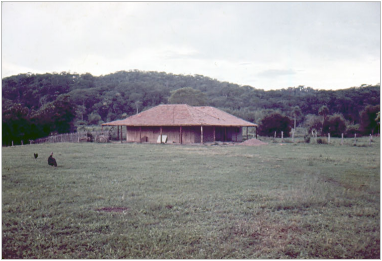
\includegraphics[width=\linewidth]{20/sede.png}
\caption{A sede da Santa Teresa.}
\end{figure}

\begin{figure}
\centering
\includegraphics[width=\linewidth]{20/águas.png}
\caption{As águas límpidas da fazenda}
\end{figure}

Enquanto esperávamos que Benício se mudasse, passamos um tempo hospedados na fazenda do Léo Brito e sua mulher Lisete, ambos agrônomos e ex-colegas do Paulo na Luiz de Queiroz.
